% Options for packages loaded elsewhere
\PassOptionsToPackage{unicode}{hyperref}
\PassOptionsToPackage{hyphens}{url}
%
\documentclass[
]{book}
\usepackage{amsmath,amssymb}
\usepackage{lmodern}
\usepackage{ifxetex,ifluatex}
\ifnum 0\ifxetex 1\fi\ifluatex 1\fi=0 % if pdftex
  \usepackage[T1]{fontenc}
  \usepackage[utf8]{inputenc}
  \usepackage{textcomp} % provide euro and other symbols
\else % if luatex or xetex
  \usepackage{unicode-math}
  \defaultfontfeatures{Scale=MatchLowercase}
  \defaultfontfeatures[\rmfamily]{Ligatures=TeX,Scale=1}
\fi
% Use upquote if available, for straight quotes in verbatim environments
\IfFileExists{upquote.sty}{\usepackage{upquote}}{}
\IfFileExists{microtype.sty}{% use microtype if available
  \usepackage[]{microtype}
  \UseMicrotypeSet[protrusion]{basicmath} % disable protrusion for tt fonts
}{}
\makeatletter
\@ifundefined{KOMAClassName}{% if non-KOMA class
  \IfFileExists{parskip.sty}{%
    \usepackage{parskip}
  }{% else
    \setlength{\parindent}{0pt}
    \setlength{\parskip}{6pt plus 2pt minus 1pt}}
}{% if KOMA class
  \KOMAoptions{parskip=half}}
\makeatother
\usepackage{xcolor}
\IfFileExists{xurl.sty}{\usepackage{xurl}}{} % add URL line breaks if available
\IfFileExists{bookmark.sty}{\usepackage{bookmark}}{\usepackage{hyperref}}
\hypersetup{
  pdftitle={Forensic Science and Statistics: Version 1.0.0},
  pdfauthor={Jeff Holt and Joseph Swetonic},
  hidelinks,
  pdfcreator={LaTeX via pandoc}}
\urlstyle{same} % disable monospaced font for URLs
\usepackage{longtable,booktabs,array}
\usepackage{calc} % for calculating minipage widths
% Correct order of tables after \paragraph or \subparagraph
\usepackage{etoolbox}
\makeatletter
\patchcmd\longtable{\par}{\if@noskipsec\mbox{}\fi\par}{}{}
\makeatother
% Allow footnotes in longtable head/foot
\IfFileExists{footnotehyper.sty}{\usepackage{footnotehyper}}{\usepackage{footnote}}
\makesavenoteenv{longtable}
\usepackage{graphicx}
\makeatletter
\def\maxwidth{\ifdim\Gin@nat@width>\linewidth\linewidth\else\Gin@nat@width\fi}
\def\maxheight{\ifdim\Gin@nat@height>\textheight\textheight\else\Gin@nat@height\fi}
\makeatother
% Scale images if necessary, so that they will not overflow the page
% margins by default, and it is still possible to overwrite the defaults
% using explicit options in \includegraphics[width, height, ...]{}
\setkeys{Gin}{width=\maxwidth,height=\maxheight,keepaspectratio}
% Set default figure placement to htbp
\makeatletter
\def\fps@figure{htbp}
\makeatother
\setlength{\emergencystretch}{3em} % prevent overfull lines
\providecommand{\tightlist}{%
  \setlength{\itemsep}{0pt}\setlength{\parskip}{0pt}}
\setcounter{secnumdepth}{5}
\usepackage{booktabs}
\usepackage{amsthm}
\makeatletter
\def\thm@space@setup{%
  \thm@preskip=8pt plus 2pt minus 4pt
  \thm@postskip=\thm@preskip
}
\makeatother
\ifluatex
  \usepackage{selnolig}  % disable illegal ligatures
\fi
\usepackage[]{natbib}
\bibliographystyle{apalike}

\title{Forensic Science and Statistics: Version 1.0.0}
\author{Jeff Holt and Joseph Swetonic}
\date{2022-01-17}

\begin{document}
\maketitle

{
\setcounter{tocdepth}{1}
\tableofcontents
}
\hypertarget{welcome}{%
\chapter{Welcome}\label{welcome}}

\textbf{This is a draft version of a work in progress. It is NOT intended for circulation.}

This book introduces statistical methods that are of use in forensic science.
In some cases the methods are currently used.
In others the methods are described but not generally in use,
although we hope that eventually they will be!

We assume that the reader has a basic understanding of mathematics, but no prior
knowledge of statistics is required.
We will provide a modest description of forensic methods, but as many of these are
highly nuanced we do not attempt to
provide a deep treatment of forensic methods here. However, when possible we will
try to provide references to more information.

There are portions of this book that borrow from the treatment of statistics
given in the online materials:

\begin{quote}
Online Statistics Education: A Multimedia Course of Study (\url{http://onlinestatbook.com/})
Project Leader: David M. Lane, Rice University
\end{quote}

This site provides a comprehensive introduction to statistics and is worth referencing when you would like additional information.
We deeply appreciate their willingness to allow the use of their work.

\hypertarget{an-introductory-example}{%
\section{An Introductory Example}\label{an-introductory-example}}

Consider the following scenario:
Suppose there is a late-night break-in at a closed convenience store.
No one is present to see the perpetrator, but there is low-quality CCTV footage.
Unfortunately, the \emph{only} thing that can be discerned from the video is the
color of the perpetrator's hair.

Now consider two possible versions of what comes next:

\textbf{Version 1}: The video shows that the perpetrator has \emph{brown} hair.
The day after the robbery, police see a person with brown hair walking down the street.
The person is arrested on suspicion of committing the break-in.

\textbf{Version 2}: The video shows that the perpetrator has \emph{green} hair. The
day after the robbery, police see a person with green hair walking down the street.
The person is arrested on suspicion of committing the break-in.

For the sake of this simplified example,
in both versions we assume that the color of the hair is the \textbf{only} reason the
police suspect the person who is arrested.

\textbf{Question}: In which version do you think it is more likely that the police have
arrested the person who committed the break-in?

Answering the question requires considering the likelihood that the police have
the correct person in both versions and deciding which is greater.
In most communities people with brown hair outnumber people with green hair,
so let's assume that is the case here. Intuitively,
it seems reasonable to expect that the likelihood of a correct arrest in Version 2 is greater
than that in Version 1:
Brown-haired people are relatively common, so in Version 1 the likelihood of
arresting the correct brown-haired person is probably low.
On the other hand, green-haired people are relatively rare, so in Version 2
the likelihood of arresting the correct person is higher.

Two important points:

\begin{enumerate}
\def\labelenumi{\arabic{enumi})}
\item
  Although the likelihood of the correct arrest is greater in Version 2
  than in Version 1 does not mean that the likelihood in Version 2 is high.
  It is possible that there are more brown-haired people than green-haired people
  while still having a lot of green-haird people, making the correct arrest
  unlikely in either case.
\item
  While the above discussion is interesting, the word ``likelihood'' is
  imprecise. Going forward we will develop ``probability'' which
  will allow us to quantify the notion of likelihood, so that we will be able
  to specify (for instance) how much more likely a correct arrest is in
  Version 1 than in Version 2.
\end{enumerate}

\hypertarget{introduction-to-probability}{%
\chapter{Introduction to Probability}\label{introduction-to-probability}}

\hypertarget{the-previous-example}{%
\section{The Previous Example}\label{the-previous-example}}

The example from the previous section involves the ``likelihood'' of arresting the
correct person based on their hair color. Here we begin the development of
``probability'' which allows us to quantify the notion of likelihood.

Let's start by providing some additional context for our example:
Suppose that the crime described takes place on an island of 1000 people.
The number of these people with each hair color is given in the table below.

\[
\begin{array}{c|c}
 \mathrm{Color} & \mathrm{Count} \\ \hline
\mathrm{Brown} & 670  \\ 
\mathrm{Blond} & 200  \\ 
\mathrm{Red} & 110  \\ 
\mathrm{Green} & 20  \\ 
\end{array}\\
\mbox{Table 1: Hair Color Counts}
\]

A \textbf{probability} is a number between 0 and 1 that provides a measure of the
likelihood that something occurs,
with a larger number indicating greater likelihood.

Suppose that we select a person from this population at random. To compute
the probability that this person has brown hair,
we take the number with brown hair and divide by the number of people:

\[\mbox{P(Brown hair)} = \frac{670}{1000} = 0.67\]

We use ``P(\ldots)'' to denote the probability of something. For instance in this case
\(\mbox{P(Brown hair)}\) = ``probability of brown hair''.

\hypertarget{sample-questions}{%
\subsection{Sample Questions}\label{sample-questions}}

Sprinkled thought this book are Sample Questions, which also play the role
of examples. In the online version, the
solutions to these questions are hidden. Before looking at the solution
(by hovering), we recommend that you try to do them yourself!

\textbf{1.} What is the probability that a randomly selected person has blond hair?

\textbf{Answer:} \(P(\text{Blond}) = \frac{200}{1000} = 0.20\).

\textbf{2.} What is the probability that a randomly selected person has red hair?

\textbf{Answer:} \(P(\text{Red}) = \frac{110}{1000} = 0.11\).

These examples are fine but do not answer the question from the previous section.
In Version 1, we have a brown-haired person on the CCTV and one of the
670 brown-haired people randomly arrested.
Thus the probability that the correct person is arrested is

\[\mbox{P(correct arrest)} = \frac{1}{670} = 0.00149\]

In Version 2 of the example we have a green-haired person on CCTV, so this
time the probability that the correct person is arrested is

\[\mbox{P(correct arrest)} = \frac{1}{20} = 0.05\]

Dividing the two probabilities

\[\frac{0.05}{0.00149} = 33.5\]

we see that a correct arrest in Version 2 is 33.5 times as likely as in Version 1.
However, even in Version 2 there is only a 0.05 probability that the police have
the correct person!

\hypertarget{sample-questions-1}{%
\subsection{Sample Questions}\label{sample-questions-1}}

\textbf{1.} Suppose CCTV shows a red-haired person committed the robbery, and that
a random red-haired person is arrested. What is the probability of a correct
arrest in this instance?

\textbf{Answer:} \(P(\text{correct arrest}) = \frac{1}{110} = 0.00909\).

\textbf{2.} Determine the number of times greater the likelihood of a correct arrest
if the culprit has red hair vs having blond hair.

\textbf{Answer:} In the case of a blond-hairded person, we have
\(P(\text{correct arrest}) = \frac{1}{200} = 0.005\). Therefore the ratio
of probabilities is
\(\frac{0.00909}{0.005} = 1.81818\)
so a correct arrest for a red-haired culprit is 1.81818 times as likely
as for a blond-haired culprit.

\hypertarget{exercises}{%
\section{Exercises}\label{exercises}}

\[\mbox{Put exercises here}\]

\hypertarget{joint-probability}{%
\chapter{Joint Probability}\label{joint-probability}}

Blood plays a role in many forensic science applications, with the ``blood
type'' determined by a combination of two different blood group systems:

\begin{quote}
\emph{Blood types are inherited and represent contributions from both parents.
As of 2019, a total of 41 human blood group systems are recognized by the
International Society of Blood Transfusion (ISBT). The two most
important blood group systems are ABO and Rh; they determine someone's
blood type (A, B, AB, and O, with +, − or null denoting RhD status)
for suitability in blood transfusion.}

Source: \url{https://en.wikipedia.org/wiki/Blood_type}
\end{quote}

\begin{figure}
\centering
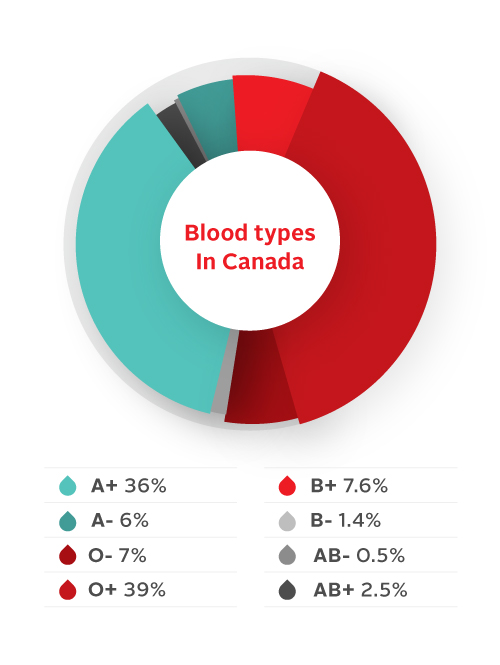
\includegraphics{images/BloodType-PieGraph_0.jpg}
\caption{Source: \url{https://www.blood.ca/en/blood/donating-blood/whats-my-blood-type}}
\end{figure}

Suppose that we have a collection of 1000 people, each classified by Rh
(Rh+ or Rh-) and ABO (A, B, AB, or O).
The number of people of each combination of Rh and ABO grouping is shown
in the table below.

\[
\begin{array}{c|c|c}
           & \mathrm{Rh+} & \mathrm{Rh-}\\ \hline
\mathrm{A} & 360 & 60 \\ 
\mathrm{B} & 76 & 14 \\ 
\mathrm{AB} & 25 & 5 \\ 
\mathrm{O} & 390 & 70 \\ 
\end{array}\\
\mbox{Rh and ABO counts}
\]

Suppose that we select one of the people at random, and note that person's groups.
There are various possibilities for outcomes, such as the person selected is Rh+ and O.
The likelihood that this combination occurs is the \textbf{joint probability} of the two classifications,
Rh and ABO grouping.
As 390 out of the 1000 people are O+, the probability of selecting such a person is

\[\mbox{P(O+)} = \frac{390}{1000} = 0.39\]

Here, P(O+) stands for the probability that the person selected is Rh+ \textbf{and} type O.
A sample of other probabilities that come directly from the table are

\[\begin{array}{rcccl}
\mbox{P(Female and Type O)} & = & {\displaystyle\frac{202}{1000}} & = & 0.202 \\[5pt]
\mbox{P(Male and Type AB)} & = & {\displaystyle\frac{24}{1000}} & = & 0.024 \\[5pt]
\mbox{P(Male and Type A)} & = & {\displaystyle\frac{235}{1000}} & = & 0.235 \\
\end{array}\]

We also can combine table entries to compute other probabilities.
For instance, there are a total of \(16 + 24 = 40\) people with blood type AB, so

\[
\mbox{P(Type AB)} = \frac{40}{1000} = 0.04
\]

For another example, there are a total of \(235 + 24 + 63 + 248 = 570\) males in our population, so

\[
\mbox{P(Male)} = \frac{570}{1000} = 0.57
\]

\hypertarget{sample-questions-2}{%
\subsection{Sample Questions}\label{sample-questions-2}}

\textbf{1.} What is the probability that the person selected is female?

\textbf{Answer:} \(P(\text{Female}) = 1 - P(\text{Male}) = 1 - 0.57 = 0.43\) This is equivalent to \((175 + 16 + 37 + 202) / 1000\).

\textbf{2.} What is the probability that the person selected is male and has type A blood and type O blood?

\textbf{Answer:} \(P(\text{Male and A and O}) = 0\).
The probability of this event occurring in the table is zero, as no men have two different types of blood.

\hypertarget{and-vs-or}{%
\section{And vs Or}\label{and-vs-or}}

Above we saw that \(\mbox{P(Female and Type A)} = 0.175\). Suppose we instead would like to know \(\mbox{P(Female or Type A)}\)?
That is, we want to know the probability that a randomly selected person is either female or has type A blood.
(Note that this group includes those who are both female \textbf{and} have type A blood.)
From our table we see that the total number in this group is \(175 + 16 + 37 + 202 + 235 = 665\) so that

\[
\mbox{P(Female or Type A)} = \frac{665}{1000} = 0.665
\]

Other combinations are also possible.
For instance, there are \(175 + 235 = 310\) people with type A blood and \(37 + 63 = 100\) people with type B blood,
so there are a total of \(310 + 100 = 410\) people that have either type A or type B blood.
Therefore, we have

\[
\mbox{P(Type A or Type B)} = \frac{410}{1000} = 0.41
\]

\hypertarget{sample-questions-3}{%
\subsection{Sample Questions}\label{sample-questions-3}}

\textbf{1.} What is the probability of selecting a female or male with type AB blood?

\textbf{Answer:} \(P(\text{(Male or Female) and AB}) = P(\text{(Male and AB) or (Female and AB)}) = (16 + 24) / 1000 = 0.04\)

\hypertarget{probability-tables}{%
\section{Probability Tables}\label{probability-tables}}

Frequently, tables provide probabilities (or percentages) instead of counts.
To make the conversion from counts to probabilities, all we do is divide each table entry by the total.
Thus, for our table, we divide each entry by 1000 to arrive at

\[
\begin{array}{c|c|c}
           & \mathrm{F} & \mathrm{M}\\ \hline
\mathrm{A} & 0.175 & 0.235 \\ 
\mathrm{AB} & 0.016 & 0.024 \\ 
\mathrm{B} & 0.037 & 0.063 \\ 
\mathrm{O} & 0.202 & 0.248 \\ 
\end{array}\\
\mbox{Gender and blood type counts}
\]

Table 2 entries give the probability of selecting each combination. For instance

\[
\mbox{P(Female and Type O)} = 0.202
\]

We can add entries in this table to compute other probabilities.\\
For example, suppose we want to compute the probability that a randomly selected person has type O blood.
Based on the table, this can happen if a person is female and has type O blood, or if a person is male and has type O blood.
Because these two groups are disjoint, we can add the probabilities to arrive at

\[
\mbox{P(Type O)} = \mbox{P(Female and Type O)} + \mbox{P(Male and Type O)}
= 0.202 + 0.248 = 0.45
\]

If instead (for instance), we want to compute P(Female) then we add the entries in the corresponding column, giving us

\[
\mbox{Pr(Female)} = 0.175 + 0.016 + 0.037 + 0.202 = 0.43 
\]

\hypertarget{conditional-probability}{%
\chapter{Conditional Probability}\label{conditional-probability}}

Now suppose that we just focus on the females in the population, which forms a subset of the population.
The probability that a randomly selected female has blood type O is an example of a \textbf{conditional probability}.

There are 430 females in the population, and 202 of those have type O blood.
Hence, the probability that female chosen at random has type O blood is

\[
\mbox{P(Type O | Female)} = \frac{202}{430} = 0.470
\]

The vertical bar in the notation is interpreted as \emph{given that}, so that \(\mbox{P(Type O | Female)}\) is read as

\[
\mbox{The probability of blood type O, given the person is female.}
\]

Conditional probabilities arise all the time when evaluating forensic evidence. Other examples of conditional probabilities:

The probability of Type AB, given that the person is male:

\[
\mbox{P(Type AB | Male)} = \frac{24}{570} = 0.042
\]

The probability the person is female, given Type B blood:

\[
\mbox{P(Female | Type B)} = \frac{37}{100} = 0.37
\]

The probability the person is male, given Type A blood:

\[
\mbox{P(Male | Type A)} = \frac{235}{410} = 0.573
\]

\hypertarget{sample-questions-4}{%
\subsection{Sample Questions}\label{sample-questions-4}}

\textbf{1.} What is the probability of blood type AB or B given the person selected is female?

\textbf{Answer:} \(P(\text{AB or B | Female}) = (16 + 37) / 430 = 0.123\)

\hypertarget{probability-rules}{%
\chapter{Probability Rules}\label{probability-rules}}

Earlier we computed the conditional probability

\[
\mbox{P(Type O | Female)} = \frac{202}{430} 
\]

The numerator 202 came from the count of Females who have blood Type B, and the denominator 430 is the total number of Females.
If we divide the numerator and denominator by 1000, then the quotient is not changed, so that

\[
\mbox{P(Type O | Female)} = \frac{202/1000}{430/1000} 
= \frac{0.202}{0.43} = \frac{\mbox{P(Type O and Female)}}{\mbox{P(Female)}}
\]

This illustrates a general property of probability: If A and B represent possible outcomes, then the probability of A given B is

\[
\mbox{P(A | B)} = \frac{\mbox{P(A and B)}}{\mbox{P(B)}}
\]

Multiplying on both sides of the above equation by P(B) gives

\[
\mbox{P(A and B)} = \mbox{P(A | B)}\mbox{P(B)}  
\]

This is called the \textbf{multiplication rule}. Reversing the order of A and B above gives

\[
\mbox{P(B and A)} = \mbox{P(B | A)}\mbox{P(A)}  
\]

In the blood type example, it is clear that P(Female and Type O) is the same as P(Type O and Female).
This is true in general: P(A and B) = P(B and A)\}, it follows that
\[
\mbox{Pr(A $|$ B)}\mbox{Pr(B)}  = \mbox{Pr(B $|$ A)}\mbox{Pr(A)} 
\]
so that
\[
\mbox{Pr(A $|$ B)}  = \mbox{Pr(B $|$ A)}\frac{\mbox{Pr(A)}}{\mbox{Pr(B)}}
\]
This formula is called \textbf{Bayes Rule}. Applied to our earlier population, we have
\[
\mbox{Pr(Type O $|$ Female)} = \mbox{Pr(Female $|$ Type O)}\frac{\mbox{Pr(Type O)}}{\mbox{Pr(Female)}}
\]

Two outcomes A and B are \textbf{independent} when \$\mbox{Pr(A $|$ B)} = \mbox{Pr(A)}\$,
which implies that knowing if B has occurred has no effect on the probability of A.

\hypertarget{counterintuitive-applications}{%
\chapter{Counterintuitive Applications}\label{counterintuitive-applications}}

\hypertarget{birthday-paradox}{%
\section{Birthday Paradox}\label{birthday-paradox}}

How many people are needed in a classroom so that the probability of them sharing a birthday is at least \(\frac{1}{2}\)?
Intuitively, one could claim that 183 people in the group would imply that the probability is greater than \(\frac{1}{2}\),
since \(\frac{183}{365} = 0.501\). However, intuition does not correctly solve this problem.

To begin, there are some assumptions that need to be made.
For simplicity, we will ignore leap years and assume that all 365 birthdays have an equal probability of occurring.

We want to compute \(P(\beta)\), the probability that at least 2 people share the same birthday.
Recall from the previous chapter that \(P(\beta) = 1 - P(\beta')\).
In this case, it is much simpler to calculate the probability that no one in the group shares the same birthday with someone else.

Let's start with the simple example involving only two people. The probability that they do not share the same birthday is
\[P(\beta') = \left( \frac{365}{365} \right) \left( \frac{364}{365} \right) = 0.997\]
\[1 - P(\beta') = 0.003\]

Extending this result to a group of five people:
\[P(\beta') = \left( \frac{365}{365} \right) \left( \frac{364}{365} \right) \left( \frac{363}{365} \right) 
\left( \frac{362}{365} \right) \left( \frac{361}{365} \right)\]
\[ = \frac{365!}{365^5(365 - 5)!} = 0.973\]
\[1 - P(\beta') = 0.027\]

This formula can be applied to any number of group size, so that in the general case of \(n\) people,
the probability that at least two share the same birthday is
\[P(\beta) = 1 - \frac{365!}{365^n(365 - n)!}\]

Finally, to solve the original question:
How many people are needed in a classroom so that the probability of them sharing a birthday is at least \(\frac{1}{2}\)?
Iteratively increasing the group size from five, it is clear to see that at a group size of 23, \(P(\beta) > \frac{1}{2}\)
\[P(\beta) = 1 - P(\beta') = 1 - \frac{365!}{365^{23}(365 - 23)!} = 0.507\]

\hypertarget{monty-hall-problem}{%
\section{Monty Hall Problem}\label{monty-hall-problem}}

The original problem was popularized as a letter by Craig F. Whitaker sent to Marilyn vos Savant's column in Parade magazine in 1990.
You can read more about the article here: \url{https://web.archive.org/web/20130121183432/http://marilynvossavant.com/game-show-problem/}

Suppose you're on a game show, and you're given the choice of three doors. Behind one door is a car, behind the others, goats.
You pick a door, say \#1, and the host, who knows what's behind the doors, opens another door, say \#3, which has a goat.
He says to you, ``Do you want to pick door \#2?'' Is it to your advantage to switch your choice of doors?

  \bibliography{book.bib,packages.bib}

\end{document}
